\documentclass[12pt,xcolor=table,aspectratio=169]{beamer}
\usetheme{Frankfurt}
\usecolortheme{rose}
\usepackage{amsthm}
\usepackage{amsmath}
\usepackage{bbm}
\usepackage{amsfonts}
\usepackage{amssymb}
\usepackage{graphicx}
\usepackage{hyperref}
\usepackage[flushleft]{threeparttable}
\usepackage{tabularx}
\usepackage{booktabs}
\usepackage{siunitx}
\usepackage{tikz}
\usetikzlibrary{decorations.pathreplacing,angles,quotes}
%\usepackage{enumitem}% http://ctan.org/pkg/enumitem

%set up course and number

\newcommand{\ClassName}{TBD}
\newcommand{\ClassNumber}{TBD}
\newcommand{\Topic}{TBD}

% Some optional colors. Change or add as you see fit.
%---------------------------------------------------
 \definecolor{ualbertagreen}{HTML}{007C41}
\definecolor{ualbertagold}{HTML}{FFDB05}

\definecolor{calloutgrey}{HTML}{D9D9D9}


%set fonts
\setbeamerfont{subtitle}{size=\large,shape=\scshape,series=\bfseries}
\setbeamerfont{title}{size=\Large,shape=\scshape,series=\bfseries}
\setbeamerfont{author}{size=\large}
\setbeamerfont{date}{size=\large}
\setbeamerfont{caption}{size=\scriptsize}


% Some optional color adjustments to Beamer. Change as you see fit.
%------------------------------------------------------------------
\setbeamercolor{frametitle}{fg=ualbertagreen,bg=white}
\setbeamercolor{title}{fg=ualbertagreen,bg=white}
\setbeamercolor{author}{fg=ualbertagreen,bg=white}
\setbeamercolor{date}{fg=ualbertagreen,bg=white}
\setbeamercolor{local structure}{fg=ualbertagreen}
\setbeamercolor{section in toc}{fg=ualbertagreen,bg=white}
% \setbeamercolor{subsection in toc}{fg=ualbertagreen,bg=white}
\setbeamercolor{footline}{fg=ualbertagreen!50, bg=white}

% definition boxes
\setbeamercolor{block title}{bg=ualbertagreen,fg=white}
\setbeamercolor{block body}{parent=normal text,use=block title,bg=calloutgrey}
%\setbeamercolor{block body}{parent=normal text,use=block title,bg=block title.bg!30!bg}


\setbeamercolor{upper separation line head}{bg=ualbertagreen}
\setbeamercolor{lower separation line head}{bg=ualbertagold}
\setbeamercolor{middle separation line head}{bg=ualbertagold}
\setbeamercolor{frametitle}{fg=ualbertagreen,bg=white}



\setbeamercolor{section in head/foot}{bg=white,fg=ualbertagreen}
\setbeamercolor{author in head/foot}{bg=white,fg=ualbertagreen}
\setbeamercolor{date in head/foot}{bg=white,,fg=ualbertagreen}
\setbeamercolor{title in head/foot}{bg=white,fg=ualbertagreen}

\setbeamercolor{headline}{bg=white,fg=ualbertagreen}




\setbeamercolor*{middle separation line head}{bg=ualbertagreen}
\setbeamercolor*{alerted text}{fg=ualbertagreen}
\setbeamercolor*{example text}{fg=black}
\setbeamercolor*{structure}{fg=black}


\let\Tiny=\tiny



\logo{
   %\ifnum\insertpagenumber>1
   \tikz [remember picture,overlay]
    \node[yshift=.3cm,xshift=1.5cm] at (current page.south west)
        %or: (current page.center)
        {
\includegraphics[width=1in]{../images/UA-ASB-COLOUR.png}};
    %\fi
%
\includegraphics[height=0.8cm]{../images/UA-ASB-COLOUR.png}\vspace{220pt}
}


\setbeamertemplate{title page}{%
  \vbox{}
    \vspace{.5cm}% NEW
  \begingroup
    \centering
    \begin{beamercolorbox}[sep=8pt,center]{title}
      \usebeamerfont{title}\ClassNumber: \ClassName\par%
      \usebeamerfont{title}\inserttitle\par%
     \ifx\insertsubtitle\@empty%
      \else%
        \vskip0.05em%
        {\usebeamerfont{subtitle}\usebeamercolor[fg]{subtitle}\insertsubtitle\par}%
      \fi%
    \end{beamercolorbox}%
    \begin{beamercolorbox}[sep=8pt,center]{author}
      \usebeamerfont{author}\insertauthor
    \end{beamercolorbox}
    \begin{beamercolorbox}[sep=8pt,center]{institute}
      \usebeamerfont{institute}\insertinstitute
    \end{beamercolorbox}

    \vspace{0.5cm}% NEW
    \begin{beamercolorbox}[sep=8pt,center]{date}
      \usebeamerfont{date}\insertdate
    \end{beamercolorbox}\vskip0.05em

      \endgroup
  %\vfill
}


\setbeamertemplate{frametitle}{%
    \insertframetitle\par\vskip-10pt
}



\renewcommand{\ClassName}{Business Economics, Organization and Management}
\renewcommand{\ClassNumber}{BUEC 311}

\setbeamertemplate{headline}{%
\leavevmode%
 \hbox{%
    \begin{beamercolorbox}[wd=\paperwidth,ht=5ex,dp=0ex]{white}%
    \usebeamerfont{headline}\hskip6pt\ClassNumber: \inserttitle\par%
    \insertsectionnavigationhorizontal{\paperwidth}{}{\hskip0pt plus1filll}
    \end{beamercolorbox}%
  }
}

\defbeamertemplate*{footline}{my footline}{%
    \ifnum\insertpagenumber=1
        \Tiny{%
            \hfill%
		\vspace*{1pt}%
            %\insertframenumber/\inserttotalframenumber \hspace*{0.1cm}%
            \newline%
            \color{ualbertagold}{\rule{\paperwidth}{0.4mm}}\newline%
            \color{ualbertagold}{\rule{\paperwidth}{.4mm}}%
        }
  \else%
        \Tiny{%
            \hspace{.66\paperwidth}
            %\vspace{25pt}
            \insertframenumber/\inserttotalframenumber
            \newline%
            \color{ualbertagold}{\rule{\paperwidth}{0.4mm}}\newline%
            \color{ualbertagold}{\rule{\paperwidth}{.4mm}}%
        }%
    \fi%
}


\newenvironment{itemize*}%
  {\begin{itemize}%
    \setlength{\itemsep}{0pt}%
    \setlength{\parskip}{0pt}}%
  {\end{itemize}}


\title{
	Producer Behaviour, Part 2
}

\date{Fall 2020}

\begin{document}

\section{Outline}

\frame{
	\titlepage
}



\frame{
	\frametitle{Outline}
	\begin{enumerate}
	\item Conceptualizing costs.
	\item[]
	\item Common measures of costs.
	\item[]
	\item Costs in the short run and long run.
	\item[]
	\item The learning curve.
	\item[]
	\item The costs of producing multiple goods.
	\end{enumerate}
}


\section{Conceptualizing Costs}

\frame{
	\frametitle{Outline}
	\begin{enumerate}
	\item \alert{Conceptualizing costs.}
	\item[]
	\item Common measures of costs.
	\item[]
	\item Costs in the short run and long run.
	\item[]
	\item The learning curve.
	\item[]
	\item The costs of producing multiple goods.
	\end{enumerate}
}

\frame{
	\frametitle{Conceptualizing Costs}
	\begin{itemize}
	\item Previously, we examined how output changes in response to changes in inputs, technology, etc.
	\item[]
	\item But the technical relationship between inputs and outputs defined by the production process is only one determinant of how firms choose what to produce.
	\item[]
	\item We also need to account for the cost of inputs.
	\end{itemize}
}

\frame{
	\frametitle{Explicit and Implicit Costs}
	\begin{itemize}
	\item Financial accounting statements correctly measure costs for tax purposes and to meet other legal requirements.
	\item[]
	\item To make sound managerial decisions, good managers need more information.
	\item[]
	\item We need to think about both \textit{explicit} and \textit{implicit} costs.
		\begin{itemize}
		\item Explicit costs are direct, out-of-pocket payments for labor, capital, energy and materials.
		\item Implicit costs reflect forgone opportunities rather than explicit, current expenditure.
		\end{itemize}
	\end{itemize}
}

\frame{
	\frametitle{Opportunity Costs}
	\begin{itemize}
	\item The \textit{opportunity cost} of a resource is the value of the best alternative use of that resource.
	\item[]
	\end{itemize}
	\begin{example}[Opportunity costs]
	Taylor owns and manages a consulting firm. The firm's monthly revenue is \$55k, and monthly costs are \$46k, which includes a \$2k per month salary for Taylor. Taylor also collects the firm's profits each month. Alternatively Taylor could work for another firm and receive \$12k per month. Given this, is Taylor using her labor effectively? Why or why not?
	\end{example}
}

\frame{
	\frametitle{Trumpian Opportunity Costs}
	\begin{figure}
	\centering
	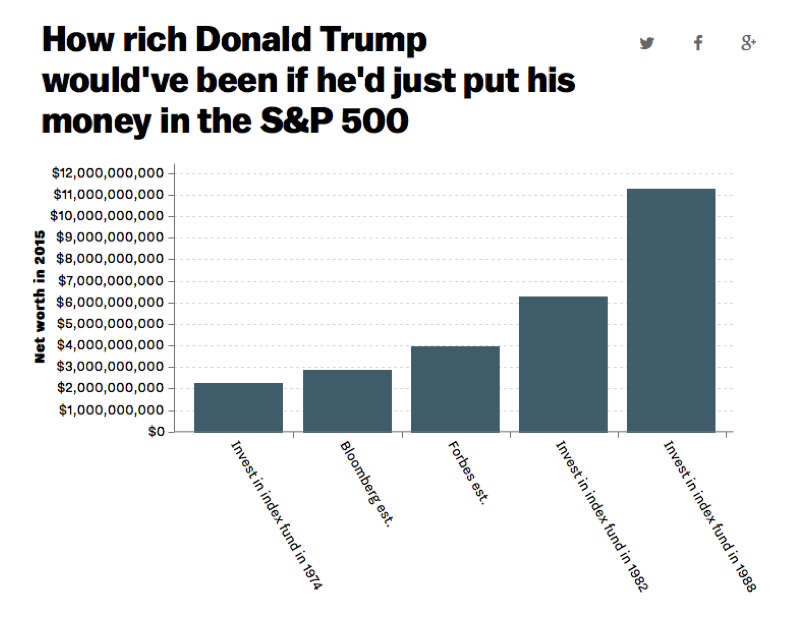
\includegraphics[scale=.6]{../images/donald.png}
	\caption{The opportunity cost of being Donald?}
	\end{figure}
}

\frame{
	\frametitle{Opportunity Costs}
	\begin{itemize}
	\item The opportunity cost for inputs that can be bought and used in the same period can be determined from the market.
		\begin{itemize}
		\item E.g: Labor services, energy, and materials.
		\end{itemize}
	\item[]
	\item It is more difficult to determine the opportunity costs of inputs that are \textit{durable}.
		\begin{itemize}
		\item Durable inputs are useable for a long period, perhaps for many years.
		\item E.g: Capital, such as land, buildings, and equipment.
		\end{itemize}
	\end{itemize}
}

\frame{
	\frametitle{Durable Input Costs}
	\begin{itemize}
	\item Two issues with durable inputs:
		\begin{enumerate}
		\item How do we allocate the initial purchase cost over time?
		\item What do we do if the value of the input changes over time?
		\end{enumerate}
	\item[]
	\item Accountant may expense input or amortize it over the life of the input following standard accounting rules.
	\item[]
	\item The decision to operate the input is independent of the expense/amortize decision; it depends on the opportunity cost of the input.
	\end{itemize}
}

\frame{
	\frametitle{Durable Input Costs}
	\begin{example}[Opportunity Costs and Durable Inputs]
	Consider the case of Tony, who is deciding on whether or not to operate a welding truck. Operating the truck earns the company \$2k per month, but the truck depreciates at a value of \$1k per month.
		\begin{enumerate}
		\item First, suppose that Tony can rent the truck to Kelly's Welding Company at a rate of \$2.25k per month. Should Tony operate the truck?
		\item Next, suppose that there is no rental market for trucks. Should Tony operate the truck?
		\end{enumerate}
	\end{example}
}

\frame{
	\frametitle{Sunk Costs}
	\begin{itemize}
	\item Some costs that appear in financial accounts are not relevant for managerial decisions.
	\item[]
	\item These are \textit{sunk costs}: past expenditures that cannot be recovered.
	\item[]
	\item Sunk costs should be ignored by managers when making decisions.
	\end{itemize}
}

\frame{
	\frametitle{Sunk Costs}
	\begin{example}[Sunk Costs]
	A.T. \& Love is a real estate developer that invested \$10 million to purchase an apartment building with the intent to renovate the building and turn the apartments into luxury condos. The renovation is expected to cost an additional \$2.5 million. However, since the initial purchase, a recession has hit, meaning demand for luxury condos has dried up. Gerald, one of A.T. \& Love's executives, suggests the company invest in the renovations anyway, given that ``We've already spent \$10 million on this thing - we might as well spend the additional \$2.5 to finish it up.'' Do you agree with Gerald's reasoning? Why or why not?
	\end{example}
}

\section{Measuring Costs}

\frame{
	\frametitle{Outline}
	\begin{enumerate}
	\item Conceptualizing costs.
	\item[]
	\item \alert{Common measures of costs.}
	\item[]
	\item Costs in the short run and long run.
	\item[]
	\item The learning curve.
	\item[]
	\item The costs of producing multiple goods.
	\end{enumerate}
}

\frame{
	\frametitle{Key Cost Measures}
	\begin{itemize}
	\item Three key cost measures for making decisions based on the opportunity cost of inputs:
		\begin{enumerate}
		\item Fixed Cost ($F$): A cost that does not vary with the level of output.
			\begin{itemize}
			\item Includes expenditures on land, office space, and other overhead.
			\item Often sunk, but not always.
			\end{itemize}
		\item[]
		\item Variable Cost ($VC$): A cost that changes as output changes.
			\begin{itemize}
			\item Refers to the cost of \textit{variable inputs}.
			\end{itemize}
		\item[]
		\item Total Cost ($C$): The sum of fixed and variable costs.
		\end{enumerate}
\item Industry-specific names may be different, e.g. sustaining capital costs.
	\end{itemize}
	\begin{align*}
	C = F + VC
	\end{align*}
}

\frame{
	\frametitle{Average Costs}
	\begin{itemize}
	\item Corresponding average cost measures:
		\begin{enumerate}
		\item Average Fixed Cost ($AFC$): $AFC=F/q$
			\begin{itemize}
			\item Falls as output rises because the fixed cost is spread over more units.
			\end{itemize}
		\item[]
		\item Average Variable Cost ($AVC$): $AVC=VC/q$
			\begin{itemize}
			\item Can rise or fall with increases in output.
			\end{itemize}
		\item[]
		\item Average Cost ($AC$): $AC=AFC+AVC$
			\begin{itemize}
			\item Also referred to as average total cost.
			\item May increase or decrease with increases in output.
			\end{itemize}
		\end{enumerate}
	\end{itemize}
}

\frame{
	\frametitle{Marginal Cost}
	\begin{itemize}
	\item Another important cost concept: \textit{Marginal Costs}
	\item[]
	\item Marginal Costs ($MC$) are the amount by which a firm's cost changes if the firm produces one more unit.
		\begin{align*}
		MC = \Delta C/\Delta q
		\end{align*}
	\item[]
	\item Marginal costs are also equal to the change in variable costs from a one-unit increase in output:
		\begin{align*}
		MC = \Delta VC / \Delta q
		\end{align*}
	\end{itemize}
}

\frame{
	\frametitle{Cost Example: Ben's Pizza Shop}
	\begin{itemize}
	\item As an example, consider Ben's Pizza shop.
	\item[]
	\item Ben is interested in understanding how his costs change as he sells more pizzas.
	\end{itemize}

}

\frame{
	\frametitle{Cost Example: Ben's Pizza Shop}
	\begin{table}
	\centering
	\resizebox{.95\linewidth}{!}{% Resize table to fit within \linewidth horizontally
	\begin{tabularx}{\textwidth}{X X X X X X X X}
	{$q$} & {$F$} & {$VC$} & {$C$} & {$MC$} & {$AFC=F/q$} & {$AVC=VC/q$} & {$AC=C/q$} \\
	\hline
	0 & 5 & 0.00 & 5.00 & & & & \\
	1 & 5 & 3.01 & 8.01 & 3.01 & 5.00 & 3.01 & 8.01 \\
	2 & 5 & 5.00 & 10.00 & 1.99 & 2.50 & 2.50 & 5.00 \\
	3 & 5 & 6.73 & 11.73 & 1.73 & 1.67 & 2.24 & 3.91 \\
	4 & 5 & 8.37 & 13.37 & 1.65 & 1.25 & 2.09 & 3.34 \\
	5 & 5 & 10.00 & 15.00 & 1.63 & 1.00 & 2.00 & 3.00 \\
	6 & 5 & 11.73 & 16.73 & 1.73 & 0.83 & 1.96 & 2.79 \\
	7 & 5 & 13.75 & 18.75 & 2.02 & 0.71 & 1.96 & 2.68 \\
	8 & 5 & 16.85 & 21.85 & 3.10 & 0.63 & 2.11 & 2.73 \\
	\end{tabularx}
	}
	\end{table}
	}

\frame{
	\frametitle{Cost Example: Ben's Pizza Shop}
	\begin{itemize}
	\item We can also illustrate the relationship between different cost measures and output graphically using cost curves.
	\end{itemize}
}

\frame{
	\frametitle{Cost Example: Ben's Pizza Shop}
\begin{figure}[t!]
	\center
	\resizebox{!}{.35\linewidth}{

	\begin{tikzpicture}
	% Draw axes
	%Y
	\draw[->] (0,0) -- (0,12) ;
	\draw[] (0,8) -- node[rotate=90, above=30pt] {\textbf{Cost, $\$$}} (0,12);
	%X
	\draw[->] (0,0) -- (15,0);
	\draw[] (14,0) -- node[below=30pt] {Quantity, \textbf{$q$, pizzas per hour}} (17,0);

	%Plot Total Output
	\draw[very thick, orange] plot[smooth, tension=.7] coordinates {(0,2.5) (16,2.55)} node[right] {{$F$}};
	\draw[very thick, blue] plot[smooth, tension=.7] coordinates {(0,0) (2,1.5) (4,2.5) (6,3.365) (8,4.185) (10,5) (12,5.865) (14,6.875) (16,8.425)} node[right] {{$VC$}};	
	\draw[very thick, purple] plot[smooth, tension=.7] coordinates {(0,2.5) (2,4) (4,5) (6,5.865) (8,6.585) (10,7.5) (12,8.365) (14,9.375) (16,10.925)} node[right] {{$C$}};	

	%5
%	\draw[fill] (11,5) circle [radius =0.1];
%	\node at (11,5.1) [above] {{f}};

	%Plot illustrative lines
%	\draw[dashed] (6,0) node[below] {{6}} -- (6,6) -- (0,6) node [left] {{60}};
%	\draw[dashed] (11,0) node[below] {{11}} -- (11,9.5) -- (0,9.5) node [left] {{95}};

	%Add axes labels
	%Origin%
	\node at (0,0) [left] {{0}};

	\end{tikzpicture}
	\begin{tikzpicture}
	% Draw axes
	%Y
	\draw[->] (0,0) -- (0,12) ;
	\draw[] (0,8) -- node[rotate=90, above=30pt] {\textbf{Cost, per unit $\$$}} (0,12);
	%X
	\draw[->] (0,0) -- (15,0);
	\draw[] (14,0) -- node[below=30pt] {Quantity, \textbf{$q$, pizzas per hour}} (17,0);

	%Plot Total Output
	\draw[very thick, red] plot[smooth, tension=.7] coordinates {(2,3.01) (4,1.99) (6,1.73) (8,1.65) (10,1.63) (12,1.73) (14,2.02) (16,3.10)} node[right] {{$MC$}};
	\draw[very thick, orange] plot[smooth, tension=.7] coordinates {(2,5) (4,2.5) (6,1.67) (8,1.25) (10,1) (12,0.83) (14,0.71) (16,0.63)} node[right] {{$AFC$}};
	\draw[very thick, blue] plot[smooth, tension=.7] coordinates {(2,3.01) (4,2.5) (6,2.24) (8,2.09) (10,2) (12,1.96) (14,1.96) (16,2.11)} node[right] {{$AVC$}};	
	\draw[very thick, purple] plot[smooth, tension=.7] coordinates {(2,8.01) (4,5) (6,3.91) (8,3.34) (10,3) (12,2.79) (14,2.68) (16,2.73)} node[right] {{$AC$}};	

	%Add axes labels
	%Origin%
	\node at (0,0) [left] {{0}};

\end{tikzpicture}
}

%\caption{Taylor's Possible Choices}
\end{figure}
}

\section{Long and short run costs}

\frame{
	\frametitle{Outline}
	\begin{enumerate}
	\item Conceptualizing costs.
	\item[]
	\item Common measures of costs.
	\item[]
	\item \alert{Costs in the short run and long run.}
	\item[]
	\item The learning curve.
	\item[]
	\item The costs of producing multiple goods.
	\end{enumerate}
}

\frame{
	\frametitle{Long run costs}
	\begin{itemize}
	\item In the short run, the production function determines the shape of a firm's cost curves for given input prices.
	\item[]
	\item Why? Consider a firm with a production function of capital and labour, with capital fixed in the short run.		\begin{itemize}
		\item In the short run, diminishing marginal returns to labor determine the shape of the production function.
		\item[]
		\item Moreover, labor is the only variable input, so $VC=wL$.
		\item[]
		\item This means that as output increases, variable costs increase more than proportionally.
			\begin{itemize}
			\item Diminishing marginal returns mean more labor is needed to produce one more unit of output.
			\end{itemize}
		\end{itemize}
	\end{itemize}
}

%\frame{
%	\frametitle{3. Costs in the Short Run and Long Run}
%\begin{figure}[t!]
%	\center
%	\resizebox{!}{.45\linewidth}{

%	\begin{tikzpicture}
	% Draw axes
	%Y
%	\draw[->] (0,0) -- (0,12) ;
%	\draw[] (0,8) -- node[rotate=90, above=30pt] {\textbf{Output, $q$}} (0,12);
	%X
%	\draw[->] (0,0) -- (18,0);
%	\draw[] (14,0) -- node[below=30pt] {VC, \textbf{$\$$}} (17,0);

	%Plot Total Output
%	\draw[very thick, black] plot[smooth, tension=.7] coordinates {(0,0) (3.01,1) (5,2) (6.73,3) (8.37,4) (10,5) (11.73,6) (13.75,7) (16.85,8)} node[right] {{$C$}};	

	%5
%	\draw[fill] (11,5) circle [radius =0.1];
%	\node at (11,5.1) [above] {{f}};

	%Plot illustrative lines
%	\draw[dashed] (6,0) node[below] {{6}} -- (6,6) -- (0,6) node [left] {{60}};
%	\draw[dashed] (11,0) node[below] {{11}} -- (11,9.5) -- (0,9.5) node [left] {{95}};

	%Add axes labels
	%Origin%
%	\node at (0,0) [left] {{0}};

%	\end{tikzpicture}
%}

%\caption{Taylor's Possible Choices}
%\end{figure}
%}


\frame{
	\frametitle{Diminishing Marginal Returns}
	\begin{itemize}
	\item Diminishing marginal returns determine the shape of the marginal cost curve.
	\item[]
	\item Recall that $MC=\Delta VC/ \Delta q$, and note that with a fixed capital stock, the change in variable cost must be the change in the cost of labor, i.e.:
		\begin{align*}
		MC = \Delta VC /\Delta q = w [ \Delta L/ \Delta q]
		\end{align*}
	\item But also, $MP_{L} = \Delta q / \Delta L$, meaning:
		\begin{align*}
		MC =  w / MP_{L}
		\end{align*}
	\item This means marginal costs and the marginal product of labor are inversely related; $MC$ falls as $MP_{L}$ increases and vice-versa.
	\end{itemize}
}

\frame{
	\frametitle{Diminishing Marginal Returns}
	\begin{itemize}
	\item Diminishing marginal returns also determine the shape of the average cost curve.
	\item[]
	\item Recall $AVC = VC/q$, and note that in the short run labor is the only variable input, so $VC = wL$. Hence, in the short run:
		\begin{align*}
		AVC = wL / q
		\end{align*}
	\item But also, $AP_{L} = q/L$, so:
		\begin{align*}
		AVC = w / AP_{L}
		\end{align*}
	\item This means that average costs and the average product of labor are inversely related; $AVC$ falls as $AP_{L}$ increase and vice versa.
	\end{itemize}
}

\frame{
	\frametitle{Diminishing Marginal Returns}
	\begin{itemize}
	\item To summarize, in the short run:
		\begin{enumerate}
		\item The costs associated with fixed inputs are fixed, while the costs from inputs that can be adjusted are variable.
		\item[]
		\item For a given set of input prices, the shapes of the variable cost curves and the marginal cost curve are determined by the production function.
		\item[]
		\item Where there are diminishing marginal returns, the variable cost and cost curves become relatively steep as output increases, so the average cost, average variable cost, and marginal cost curves rise with output.
		\item[]
		\item The average cost and average variable cost curves fall when marginal cost is below them and rise when marginal cost is above them, so the marginal cost cuts both these average cost curves at their minimum points.
		\end{enumerate}
	\end{itemize}
}

\frame{
	\frametitle{Long Run Costs}
	\begin{itemize}
	\item In the long run, firms adjust all of their inputs so that the cost of production is as low as possible.
		\begin{itemize}
		\item Firms can adjust plant size, design, build new machines, and otherwise adjust inputs that were fixed in the short run.
		\item Fixed costs are \textit{avoidable} in the long run.
			\begin{itemize}
			\item These costs are no longer sunk, as in the short run.
			\end{itemize}
		\end{itemize}
	\end{itemize}
}

\frame{
	\frametitle{Long Run Costs}
	\begin{itemize}
	\item In the long run, the firm's problem becomes one of choosing between bundles of inputs.
	\item[]
	\item \underline{Recall}: In the long run, the firm can choose to produce a given quantity of output from many different \textit{technically efficient} combinations of inputs.
	\item[]
	\item So the question becomes:
		\begin{itemize}
		\item Which technically efficient combination of inputs should the firm choose?
		\end{itemize}
	\end{itemize}
}

\frame{
	\frametitle{Cost Minimization}
	\begin{itemize}
	\item \underline{Goal}: Choose the combination of inputs that is \textit{economically efficient}.
	\item[]
	\item \underline{Getting there}: Need information about the firm's production process, and information about the cost of production.
	\end{itemize}	
}

\frame{
	\frametitle{Cost Minimization}
	\begin{itemize}
	\item Suppose capital and labor are the only inputs used by the firm. In this case, the firm's total costs are given by:
		\begin{align*}
		C = w L + r K
		\end{align*}
		where $w$ is the wage rate, and $r$ is the rental rate on capital.
	\item[]
	\item The \textit{isocost line} is all of the combinations of labor and capital that have the same total cost, $\bar{C}$:
		\begin{align*}
		\bar{C} = wL + rK
		\end{align*}
	\end{itemize}
}

\frame{
	\frametitle{Cost Minimization}
	\begin{itemize}
	\item Consider the case of Axel, who is opening a new ice cream shop.
	\item[]
	\item Given that capital and labor are variable, Axel can choose between many possible input combinations.
	\item[]
	\item Suppose that Axel has \$150 to spend on inputs, labor costs 25 dollars per day ($w=\$25$), and capital costs 25 dollars per day ($r=\$25$).
	\end{itemize}
	}

\frame{
	\frametitle{Cost Minimization}
	\begin{table}
	\centering
	\resizebox{.95\linewidth}{!}{% Resize table to fit within \linewidth horizontally
	\begin{tabularx}{\textwidth}{l X X X X X }
	{Bundle} & {$L$} & {$K$} & {$wL$} & {$rK$} & {$wL+rK$} \\
	\hline
	a & 6 & 0 & \$150 & \$0 & \$150\\
	b & 5 & 1 & \$125 & \$25 & \$150\\
	c & 4 & 2 & \$100 & \$50 & \$150\\
	d & 3 & 3 & \$75 & \$75 & \$150\\
	e & 2 & 4 & \$50 & \$100 & \$150\\
	f & 1 & 5 & \$25 & \$125 & \$150\\
	g & 0 & 6 & \$0 & \$150 & \$150\\
	\end{tabularx}
	}
	\end{table}}

\frame{
	\frametitle{Cost Minimization}
	\begin{itemize}
	\item We can also present the same information graphically by rewriting the isocost line as:
		\begin{align*}
		K = \frac{\bar{C}}{r} - \frac{w}{r} L
		\end{align*}
	\end{itemize}
}

\frame{
	\frametitle{Cost Minimization}
	\begin{figure}[t!]
	\center
	\resizebox{!}{.5\linewidth}{

	\begin{tikzpicture}
	% Draw axes
	%Y
	\draw[->] (0,0) -- (0,12) ;
	\draw[] (0,8) -- node[rotate=90, above=30pt] {\textbf{$K$, Units of capital per day}} (0,10);
	%X
	\draw[->] (0,0) -- (15,0);
	\draw[] (14,0) -- node[below=30pt] {\textbf{$L$, Workers per day}} (14,0);

	% Plot Isoquants
%	\draw[color=blue, very thick, domain=0.75:12] plot (\x,{(1/\x)*(11.3/4)^(2)}) node [right] {{$q=11.3$}};
	\draw[color=red, very thick] (0,6) -- (6,0) node[above right] {{\$150 Isocost}};
	\draw[color=red, very thick, dashed] (0,10) -- (10,0)  node[above right] {{\$250 Isocost}};
	\draw[color=red, very thick, dashed] (0,3) -- (3,0) node[above right] {{\$75 Isocost}};
%	\draw[fill] (11,5) circle [radius =0.1];
%	\node at (11,5.1) [above] {{f}};

	%Plot illustrative lines
	\draw (6,0) node[below] {{6}};
	\draw[fill] (6,0) circle [radius =0.1];
	\draw (5,0) node[below] {{5}};
	\draw (0,1) node [left] {{1}};
	\draw[fill] (5,1) circle [radius =0.1];
	\draw (4,0) node[below] {{4}};
	\draw (0,2) node [left] {{2}};
	\draw[fill] (4,2) circle [radius =0.1];
	\draw (3,0) node[below] {{3}};
	\draw (0,3) node [left] {{3}};
	\draw[fill] (3,3) circle [radius =0.1];
	\draw (2,0) node[below] {{2}};
	\draw (0,4) node [left] {{4}};
	\draw[fill] (2,4) circle [radius =0.1];
	\draw (1,0) node[below] {{1}};
	\draw (0,5) node [left] {{5}};
	\draw[fill] (1,5) circle [radius =0.1];
	\draw (0,6) node[left] {{6}};
	\draw[fill] (0,6) circle [radius =0.1];
	%Add axes labels
	%Origin%
	\node at (0,0) [left] {{0}};

	\end{tikzpicture}
	}
	\end{figure}
}

\frame{
	\frametitle{Isocost lines}
	\begin{itemize}
	\item Three key properties of isocost lines:
		\begin{enumerate}
		\item The point at which the isocost line hits the capital and labor axes depends on the firm’s cost and on the price of inputs.
		\item Isocost lines that are farther from the origin have higher costs than those closer to the origin.
		\item The slope of each isocost line is the same, and is given by:
			\begin{align*}
			\frac{\Delta K}{\Delta L} = - \frac{w}{r}
			\end{align*}
		This is the rate at which the firm can trade capital for labor in input markets.
		\end{enumerate}
	\end{itemize}

}

\frame{
	\frametitle{Cost Minimization}
	\begin{itemize}
	\item We can determine the economically efficient level of production for a firm by using the information contained in an isoquant and the information contained in an isocost line.
		\begin{itemize}
		\item Isoquant $\implies$ how technology allows the firm to trade off labor and capital to produce output.
		\item Isocost $\implies$ how the firm is able to trade off labor and capital in the market.
		\end{itemize}
	\item[]
	\item The economically efficient outcome occurs when these trade-offs are the same.
		\begin{itemize}
		\item This minimizes the cost of production.
		\item Occurs when the firm chooses the combination of inputs that is on the lowest isocost line that touches the isoquant with the desired level of produciton.
		\end{itemize}
	\end{itemize}
}

\frame{
	\frametitle{Cost Minimization}
	\begin{figure}[t!]
	\center
	\resizebox{!}{.5\linewidth}{

	\begin{tikzpicture}
	% Draw axes
	%Y
	\draw[->] (0,0) -- (0,12) ;
	\draw[] (0,8) -- node[rotate=90, above=30pt] {\textbf{$K$, Units of capital per day}} (0,10);
	%X
	\draw[->] (0,0) -- (15,0);
	\draw[] (14,0) -- node[below=30pt] {\textbf{$L$, Workers per day}} (14,0);

	% Plot Isoquants
	\draw[color=blue, very thick, domain=0.75:12] plot (\x,{(1/\x)*(12/4)^(2)}) node [right] {{$q=12$}};
	\draw[color=red, very thick] (0,6) -- (6,0) node[above right] {{\$150 Isocost}};
	\draw[color=red, very thick] (0,10) -- (10,0)  node[above right] {{\$250 Isocost}};
	\draw[color=red, very thick] (0,3) -- (3,0) node[above right] {{\$75 Isocost}};

	\draw[fill] (1.05,8.95) circle [radius =0.1];
	\node at (1.05,8.95) [above right] {{b}};

	\draw[fill] (2,1) circle [radius =0.1];
	\node at (2,1) [above right] {{c}};

	%Plot illustrative lines
	\draw[dashed] (3,0) node[below] {{3}} -- (3,3)-- (0,3) node [left] {{3}};
	\draw[fill] (3,3) circle [radius =0.1] node[above right] {{a}};
	%Add axes labels
	%Origin%
	\node at (0,0) [left] {{0}};

	\end{tikzpicture}
	}
	\end{figure}
}

\frame{
	\frametitle{Cost Minimization}
	\begin{itemize}
	\item There are three equivalent rules for minimizing costs in the long run:
		\begin{enumerate}
		\item The Lowest Isocost Rule
			\begin{itemize}
			\item The firm minimizes its cost by using the combination of inputs on the isoquant that is on the lowest isocost line that touches the isoquant.
			\end{itemize}
		\item[]
		\item The Tangency Rule: $MRTS = - w/r$
			\begin{itemize}
			\item At the minimum-cost bundle, $x$, the isoquant is tangent to the isocost line. The slope of the isoquant (MRTS) and the slope of the isocost are equal.
			\end{itemize}
		\item[]
		\item The Last-Dollar Rule: $MP_{L}/w = MP_{K}/r$
			\begin{itemize}
			\item Cost is minimized if inputs are chosen so that the last dollar spent on labor adds as much extra output as the last dollar spent on capital. Thus, spending one more dollar on labor at x gets the firm as much extra output as spending the same amount on capital.
			\end{itemize}
		\end{enumerate}
	\end{itemize}
}

\frame{
	\frametitle{Cost minimization when input prices change}
	\begin{itemize}
	\item Key question: How should a firm change its behavior if the cost of one of its inputs changes?
	\item[]
	\item As an example, consider the effects of a change in the price of labor on Axel's choice of inputs given that he is producing $q=12$.
	\item[]
	\item Specifically, suppose that the cost of labor falls from \$25 to \$10.
	\end{itemize}
}

\frame{
	\frametitle{Cost minimization when input prices change}
	\begin{figure}[t!]
	\center
	\resizebox{!}{.5\linewidth}{

	\begin{tikzpicture}
	% Draw axes
	%Y
	\draw[->] (0,0) -- (0,12) ;
	\draw[] (0,8) -- node[rotate=90, above=30pt] {\textbf{$K$, Units of capital per day}} (0,10);
	%X
	\draw[->] (0,0) -- (15,0);
	\draw[] (14,0) -- node[below=30pt] {\textbf{$L$, Workers per day}} (14,0);


	% Plot Isoquants
	\draw[color=blue, very thick, domain=0.75:12] plot (\x,{(1/\x)*(12/4)^(2)}) node [right] {{$q=12$}};
	\draw[color=red, very thick] (0,6) -- (6,0) node[above right] {{\$150 Isocost}};
	\draw[color=red, very thick, domain=0:9.5 ] plot (\x,{(95/25)-10/25*\x})  node[above right] {{\$95 Isocost}};

	\draw[fill] (4.9,1.85) circle [radius =0.1];
	\node at (4.9,1.85) [above right] {{b}};

	\draw[->] (1,4.5) -- (1,3.75);
	\draw[->] (5,1.25) -- (6,1.25);

	%Plot illustrative lines
%	\draw[dashed] (3,0) node[below] {{3}} -- (3,3)-- (0,3) node [left] {{3}};
	\draw[fill] (3,3) circle [radius =0.1] node[above right] {{a}};
	%Add axes labels
	%Origin%
	\node at (0,0) [left] {{0}};

	\end{tikzpicture}
	}
	\end{figure}}

\frame{
	\frametitle{Cost minimization when input prices change}
	\begin{itemize}
	\item As in the short-run, the shape of the long-run cost curve depends on the shape of the production function.
	\item[]
	\item However, unlike the short run, where key determinant was diminishing marginal returns, in the long run, the key determinant is returns to scale.
	\end{itemize}	
}

\frame{
	\frametitle{Long Run Average Costs}	
	\begin{itemize}
	\item The Long-Run Average Cost (LRAC) curve must be U-shaped if a production function has:
		\begin{itemize}
		\item increasing returns to scale at low levels of output,
		\item constant returns to scale at intermediate levels of output, and
		\item decreasing returns to scale at high levels of output.
		\end{itemize}
	\item[]
	\item The shape of the LRAC curve can have different shapes depending on whether the production process exhibits economies of scale or diseconomies of scale.
		\begin{itemize}
		\item \textit{Economies of scale} occur if average costs fall as output expands.
		\item \textit{Diseconomies of scale} occur if average costs rise as output expands.
		\item There are \textit{no economies of scale} if average costs do not change with output.
		\end{itemize}
	\end{itemize}
}

\frame{
	\frametitle{Long Run Average Costs}	
	\begin{itemize}
	\item The shape of the LRAC curve also depends on market structure.
		\begin{itemize}
		\item In perfectly competitive markets, firms typically have U-shaped LRAC curves.
		\item[]
		\item In non-competitive markets, curves may be U-shaped, L-shaped, everywhere downward sloping, everywhere upward sloping or have other shapes.
		\end{itemize}
	\end{itemize}
}

\frame{
	\frametitle{Long Run Average Costs}	
	\begin{itemize}
	\item It is important to note that the short-run and long-run average cost curves are related.
	\item[]
	\item Specifically, long-run average costs are always equal to or below short-run average costs.
	\item[]
	\item Why is this?
	\end{itemize}
}

\frame{
	\frametitle{Long Run Average Costs}	
	\begin{figure}
	\centering
	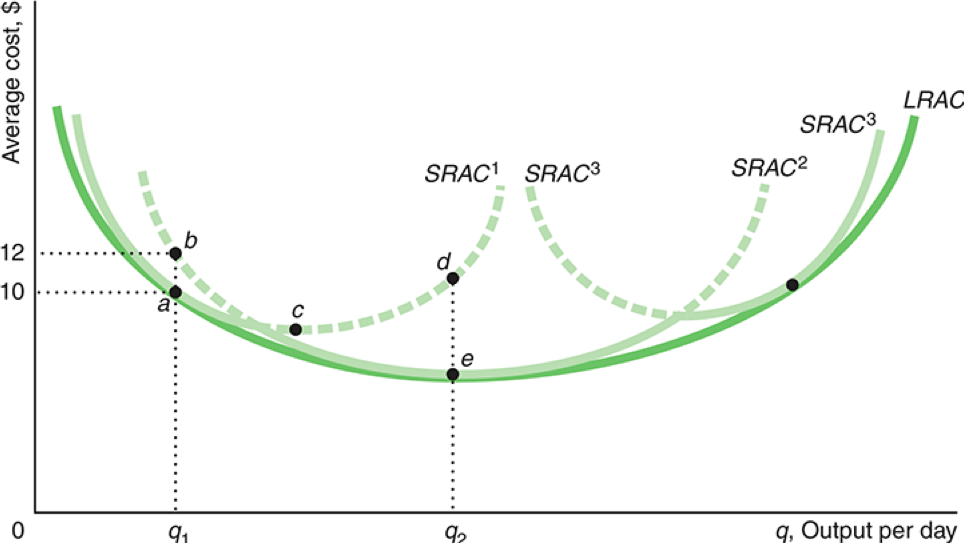
\includegraphics[scale=.6]{../images/lrac_vs_srac.png}
	\end{figure}
	}

\frame{
	\frametitle{Outline}
	\begin{enumerate}
	\item Conceptualizing costs.
	\item[]
	\item Common measures of costs.
	\item[]
	\item Costs in the short run and long run.
	\item[]
	\item \alert{The learning curve.}
	\item[]
	\item The costs of producing multiple goods.
	\end{enumerate}
}

\section{The Learning Curve}

\frame{
	\frametitle{Cost declines}
	\begin{itemize}
	\item A firm's costs may fall over time because of increasing returns to scale, technological progress, and learning by doing.
	\item[]
	\item \underline{Learning by doing} refers to the productive skills and knowledge that workers and managers gain from experience.
		\begin{itemize}
		\item Workers add speed via practice.
		\item Managers learn how to organize production more efficiently, assign tasks based on worker’s skills, and reduce inventory costs.	
		\item Engineers optimize product designs with experimentation.
		\end{itemize}
	\item[]
	\item Learning by doing tends to cause the average cost of production to fall over time as output increases.
		\begin{itemize}
		\item The effect is particularly strong with new products.
		\end{itemize}
	\end{itemize}
}

\frame{
	\frametitle{The Learning Curve}
	\begin{itemize}
	\item We can illustrate the relationship between average costs and cumulative output (the total number of units that have been produced since a product was introduced) with the \underline{learning curve}.
	\end{itemize}
}

\frame{
	\frametitle{Moore's Law}
	\begin{figure}
	\centering
	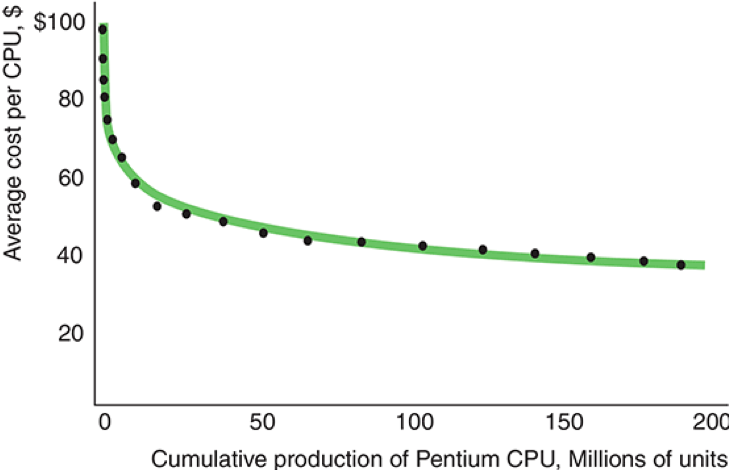
\includegraphics[scale=.6]{../images/learning_curve.png}
	\caption{Learning by Doing in Computer Chip Production}
	\end{figure}
	}

\frame{
	\frametitle{Learning-by-doing and economies of scale}
	\begin{itemize}
	\item It is important to note that the effects of learning by doing can interact with economies of scale.
	\end{itemize}
}

\frame{
	\frametitle{Learning-by-doing and economies of scale}
	\begin{figure}
	\centering
	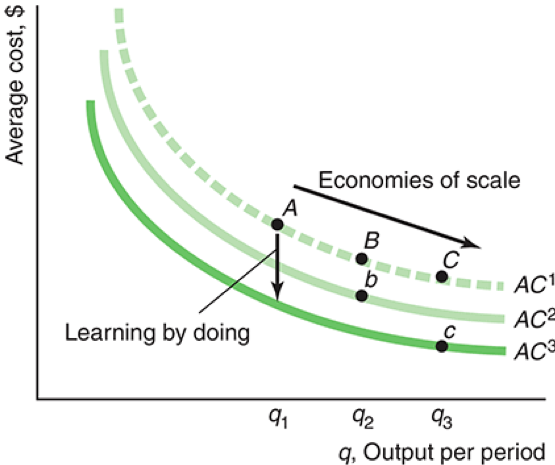
\includegraphics[scale=.6]{../images/learning_curve_with_eos.png}
	\caption{Learning by Doing with Economies of Scale}
	\end{figure}
	}


\section{Multiple goods and returns to scope}

\frame{
	\frametitle{Outline}
	\begin{enumerate}
	\item Conceptualizing costs.
	\item[]
	\item Common measures of costs.
	\item[]
	\item Costs in the short run and long run.
	\item[]
	\item The learning curve.
	\item[]
	\item \alert{The costs of producing multiple goods.}
	\end{enumerate}
}

\frame{
	\frametitle{The Cost of Producing Multiple Goods}
	\begin{itemize}
	\item If a firm produces two or more goods that are linked by a single input, the cost of one good may depend on the output level of another good.
		\begin{itemize}
		\item E.g. Cattle, oil refining.
		\end{itemize}
	\item[]
	\item Firm costs exhibit economies of scope if it is less expensive to produce goods jointly than separately.
		\begin{itemize}
		\item It is less expensive to produce beef and hides together, so there are economies of scope.
		\item It is less expensive to produce gasoline, diesel, bunker fuel, etc. together, so there are economies of scope.
		\end{itemize}
	\end{itemize}
}

\frame{
	\frametitle{The Cost of Producing Multiple Goods}
	\begin{itemize}
	\item For a production process with two outputs, the degree of scope is given by:
		\begin{align*}
		SC = \frac{[C(q_{1},0) + C(0,q_{2}) - C(q_{1},q_{2})]}{C(q_{1},q_{2})}
		\end{align*}
	where the costs of only producing $q_{1}$, of only producing $q_{2}$ and of producing both goods are given by $C(q_{1},0)$, $C(0,q_{2})$, and $C(q_{1},q_{2})$.
	\item[]
	\item $SC$ measures the percentage change in costs from producing goods jointly vs separately.
		\begin{itemize}
		\item If $SC>0$ it is cheaper to produce goods jointly, meaning there are economies of scope.
		\item If $SC<0$ it is cheaper to produce goods separately, meaning there are diseconomies of scope.
		\end{itemize}
	\end{itemize}
}

\frame{
	\frametitle{Part 2: Takeaways}
	\begin{enumerate}
	\item Good management decisions are based on opportunity cost.
	\item[]
	\item In the short run, the relationship between costs and output is determined by fixed costs and diminishing marginal returns.
	\item[]
	\item Costs are minimized in the long run by using the last dollar rule.
	\item[]
	\item In the long run, the relationship between costs and output is determined by returns to scale.
	\item[]
	\item Costs may also be influenced by learning by doing and economies of scope.
	\end{enumerate}
}

\end{document}
